\documentclass{article}
\usepackage{multimedia}
\usepackage{polski}
\usepackage[utf8]{inputenc}
\usepackage[T1]{fontenc}
\usepackage{color}
\usepackage{amsthm}
\usepackage{graphicx}
\usepackage{float}
\usepackage{afterpage}

\renewcommand*{\figurename}{\textit{Rysunek}}
\renewcommand{\thefigure}{\textit{\arabic{figure}}}
\renewcommand*{\tablename}{\textit{Tabela}}
\renewcommand{\thetable}{\textit{\arabic{figure}}}


\begin{document}

\begin{titlepage}
	\vspace{2em}{\centering\large{Instytut Informatyki Uniwersytetu Wrocławskiego}\par}

  \vspace{17em}{\centering\large{Agnieszka Dudek, Piotr Kowalczyk}\par}

	\vspace{2em}{\centering\huge{Dokumentacja projektu Tablica efektów kształcenia}\par}

	\vspace{4em}{\centering\Large{Koncepcja wykonania systemu}\par}

	\vspace{17em}{\centering\large{Wrocław, \today}\par}

	\vspace{1em}{\centering\large{Wersja 0.2}\par}

\end{titlepage}

\addtocounter{page}{1}
\newpage

\begin{table}[h!]
	\begin{center}
		\caption{Historia zmian dokonywanych w dokumencie}
		\begin{tabular}{|l|l|l|l|}
			\hline
			Data & Numer wersji & Opis & Autor \\
			\hline \hline
			2018-11-26 & 0.1 & Utworzenie dokumentu & Piotr Kowalczyk \\
			\hline 
			2018-12-01 & 0.2 & Korekta dokumentu & Agnieszka Dudek \\
			\hline
	      \end{tabular}
	\end{center}
\end{table}	

\tableofcontents

\newpage


\section{Wprowadzenie}

\subsection{Cel dokumentu}
Niniejszy dokument ma na celu precyzyjny opis koncepcji wykonania projektu \textit{Tablica efektów kształcenia}.
Stworzony jest na potrzeby przedmiotu inżynieria oprogramowania.


\section{Scenariusze przypadków użycia}
Dla trzech historyjek użytkownika przedstawionych w dokumencie Specyfikacja wymagań opisujemy dokładne scenariusze dialogu człowieka z komputerem.

\subsection{Pierwszy scenariusz}
Po zalogowaniu do Systemu Zapisów widoczny jest przycisk podpisany \textit{Tablica efektów} (dalej zwany przyciskiem). 
Znajduje się on za przyciskami \textit{Pracownicy} i \textit{Studenci}. Po kliknięciu przycisku wyświetla się ekran, na którym znajdują się:
\begin{itemize}
	\item lista dotychczas zrealizowanych efektów kształcenia,
	\item lista efektów kształcenia czekających na zrealizowanie,
	\item lista punktów ECTS zdobytych z poszczególnych grup przedmiotów.
\end{itemize}
Student może skupić uwagę na trzeciej z wymienionych list lub wydrukować wszystkie dane.

\subsection{Drugi scenariusz}
Analogicznie do pierwszego scenariuszu studentka po kliknięciu przycisku \textit{Tablica efektów} dostaje listy zrealizowanych i niezrealizowanych efektów kształcenia.
Może przewijać listę efektów kształcenia czekających na zrealizowanie i sprawdzić, czy uda jej się wszystkie wymagania spełnić w kolejnym semestrze.

\subsection{Trzeci scenariusz}
Zmiana przedmiotu w USOSie powoduje, że w następnej migracji danych aktualizowane są dane w Systemie Zapisów dotyczące efektów kształcenia.

\newpage

\section{Projekty ekranów dla przypadków użycia}
\subsection{Pierwszy scenariusz}
\begin{figure}[H]
	\begin{center}
		\caption{Projekt przycisku \textit{Tablica efektów}}
		
\includegraphics[scale=0.5]{te.png}
	\end{center}
\end{figure}

\begin{figure}[H]
	\begin{center}
		\caption{Projekt list zrealizowanych efektów}
		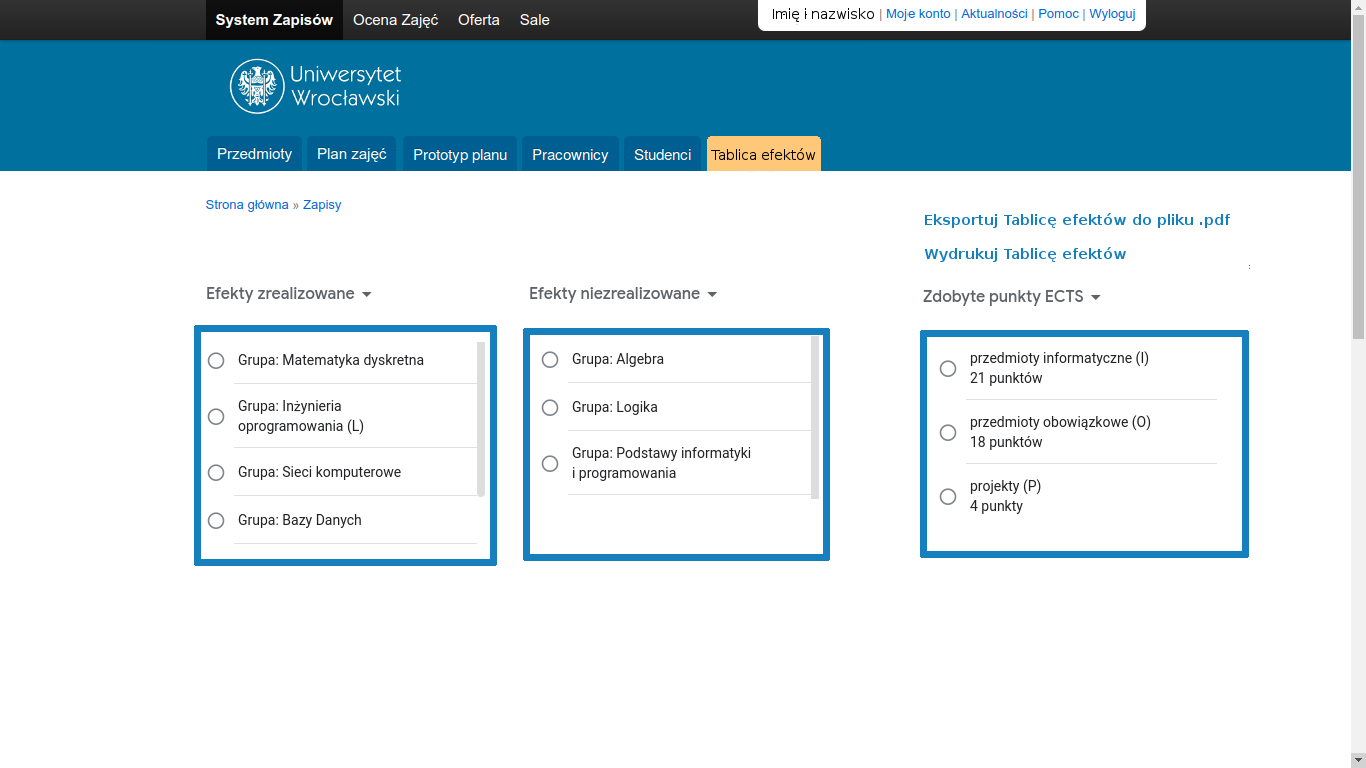
\includegraphics[scale=0.23]{tabl.png}
	\end{center}
\end{figure}

\subsection{Drugi scenariusz}
\begin{figure}[H]
	\begin{center}
		\caption{Projekt rozwijania poszczególnych list}
		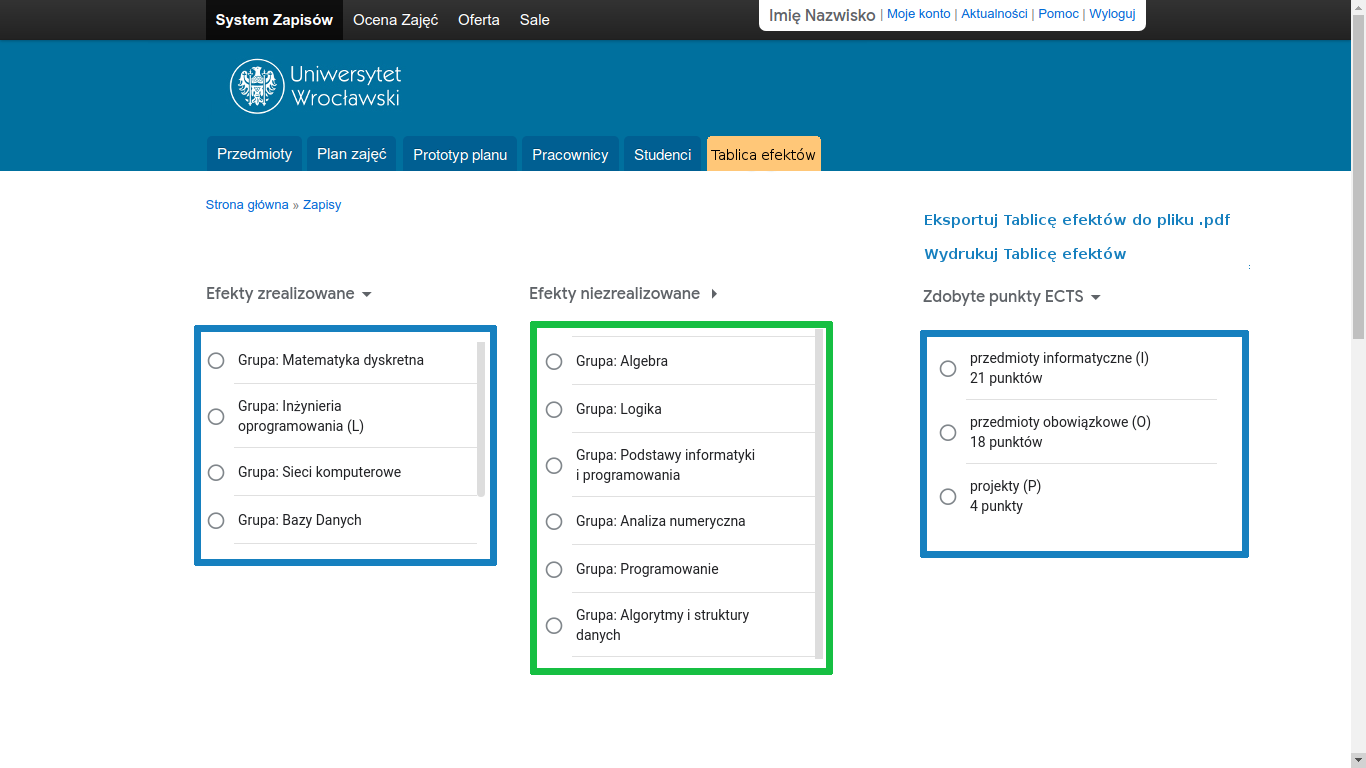
\includegraphics[scale=0.23]{rozwin.png}
	\end{center}
\end{figure}

\subsection{Trzeci scenariusz}
\begin{figure}[H]
	\begin{center}
		\caption{Projekt list w trybie edycji ręcznej}
		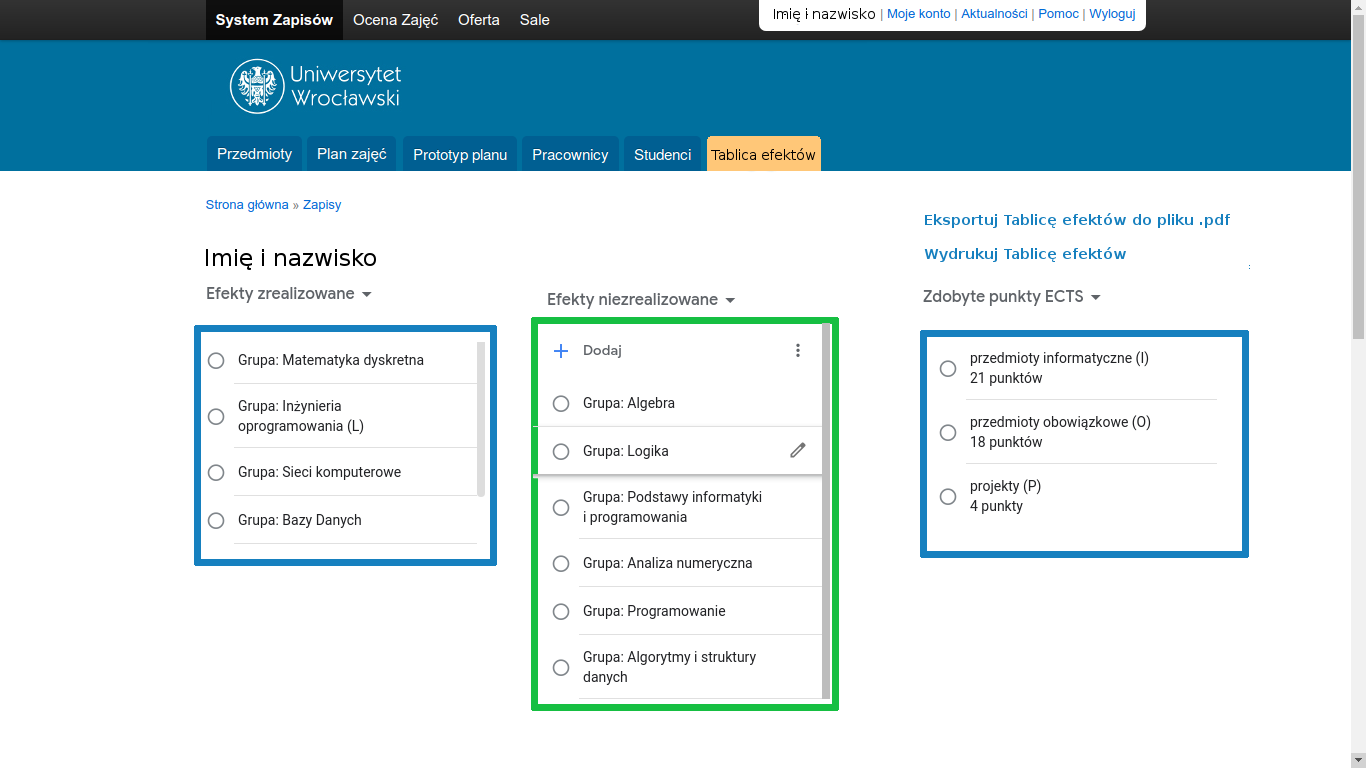
\includegraphics[scale=0.23]{edycja.png}
	\end{center}
\end{figure}


\section{Projekt architektury}

\subsection{Model konceptualny rzeczywistości, której dotyczy nasza~aplikacja}
Obiekty świata rzeczywistego:
\begin{itemize}
 \item student [imię, nazwisko, numer indeksu, tok studiów],
 \item efekt kształcenia [nazwa, tok studiów, zrealizowanie],
 \item grupa przedmiotów [nazwa, tok studiów, liczba zdobytych punktów].
\end{itemize}
Związki binarne o typie asocjacji 1:M :
\begin{itemize}
 \item student posiada efekt kształcenia [obowiązkowe ze strony studenta],
 \item student zbiera punkty w grupie przedmiotów [opcjonalne ze strony studenta].
\end{itemize}

\subsection{Podstawowe elementy aplikacji}
\begin{itemize}
 \item aplikacja będzie częścią serwisu System Zapisów,
 \item aplikacja będzie używać bazy danych,
 \item do napisania aplikacji będziemy używać zintegrowanego środowiska programistycznego Eclipse,
 \item aby przetestować aplikację skorzystamy z oprogramowania TestRail.
\end{itemize}

\subsection{Omówienie interfejsów aplikacji z otoczeniem}
Głównym interfejsem aplikacji jest strona Systemu Zapisów. Oprócz tego ważne jest powiązanie z USOSem. Jest także furtka, służąca do ręcznych poprawek w sytuacjach wyjątkowych (takich, które nie są skorelowane ze zmianami w USOSie).

\section{Schemat bazy danych}
Baza danych składa się z tylu tablic, ile jest toków studiów na kierunku informatyka na naszej uczelni. Kluczami są identyfikatory studentów, a efekty kształcenia kolejnymi polami typu boolean lub integer (nie da się być jednocześnie na dwóch tokach studiów).

Baza jest tworzona (za pierwszym razem) i aktualizowana podczas migracji danych z USOSa.

\section{Zasady kodowania}
Podczas kodowania będą obowiązywać zasady z Systemu Zapisów, a przypadki tamże niezdefiniowane rozstrzygane będą zgodnie z normą wypracowaną przez Google\footnote{https://google.github.io/styleguide/jsguide.html}.

\section{Ryzyko}

\subsection{Identyfikacja ryzyka}
Nie musimy się bać, że nasze oprogramowanie przestanie być potrzebne. Nie musimy się bać, że stracimy odbiorców. Ale za to wykonanie projektu może się opóźnić i tego się głównie boimy.
Musimy również pokazać naszym odbiorcom, że jesteśmy wiarygodni. Nasze dane od początku muszą być kompletne i prawdziwe, w przeciwnym wypadku stracimy zaufanie studentów.

\subsection{Zasady zarządzania ryzykiem}
Aby zapewnić kompletność danych, musimy skonsultować się z osobami odpowiedzialnymi za system efektów kształcenia na naszej uczelni oraz pracownikami dziekanatu, którzy odpowiadają
za aktualizowanie danych. Ważne jest również dogłębne przetestowanie naszego produktu, aby mieć pewność, że wyświetlane dane są zawsze poprawne.

Żeby zdążyć z projektem do końca semestru letniego musimy trzymać się harmonogramu od początku realizacji projektu. Dodatkowo już na początku możemy skontaktować się z osobami, 
na których konsultacjach będzie nam zależeć.


\section{Ocena zgodności wykonanych prac z planami}
Ostatnim etapem pracy będzie porównanie osiągniętych efektów z planami. Głównym celem naszego projektu jest dostarczanie danych o zrealizowanych efektach kształcenia.
Dopuszczamy zmianę ostatecznego wyglądu strony oraz podziału informacji na listy, jednak nie możemy zmienić zakresu wyświetlanych danych.

\end{document}
